%=========================================================================
% fig-opts-loop-access.tex
%=========================================================================

\begin{figure}[b]

  \centering
  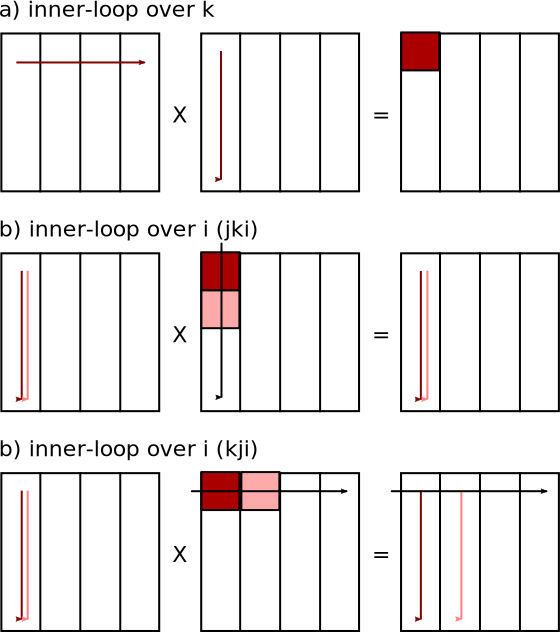
\includegraphics[width=0.5\tw]{fig-opts-loop-access.svg.pdf}

  \caption{\textbf{Memory Access Patterns of Loop Orderings --} The
    memory access patterns for the innermost loop for {\tt{ijk}},
    {\tt{jki}}, and {\tt{kji}} orderings are shown in dark red. For the
    latter two orderings, the light red arrows show the change in the
    accesses with each iteration of the middle loop. Note that {\tt{jki}}
    can reuse the data in the cache for both {\tt{B}} and {\tt{C}},
    whereas {\tt{kji}} can only reuse the data in the cache for
    {\tt{A}}. }

  \label{fig-opts-loop-access}

\end{figure}
